\section{Trading Environment}
We build a trading environment compatible with Open AI Gym \cite{brockman2016openai} that serves two primary goals. The first objective is to translate domain-specific inputs into state/reward as inputs to the RL model. The second goal is to build the portfolio from the output of the RL model, the action.

\par
The observable state S will be an n dimension vector space of real numbers between -1 and 1, where n is the number of features.
\[
    S = \{ {s \in \mathbb{R} | -1 \leq s \leq 1 } \} ^n
\]

\par
The reward R will be a real number without any other constraint.
\[
    R \in \mathbb{R}
\]
The trading environment will represent the portfolio W in an m dimension vector space of real numbers between 0 and 1 with the sum equal to 1, where m is the number of investments in the investment universe.
\[
    W = \{ {w \in \mathbb{R} | 0 \leq s \leq 1 } \} ^m,
    \\
    \sum_{i=1}^m {w_i} =1
\]
\par
The trading environment contains few components, State Extractor, Portfolio Builder, Trading System, and the Reward Provider to archive its objectives.

\subsection {State Extractor}
The State Extract extracts states from the features. 
The first steps is to normalize the input features to mean 0 and standard division \(Scale_{state}\),
\[
    f^{'}_{n,t} = \frac{f_{n,t} -  mean(f_n)}{VAR(f_n)}*Scale_{state} 
\]

During experiment, we observed the difference of performance , in terms of CAGR, between training and validation is significant. As we assume over-fit is one of the cause, we include a normal distributed noise \(\mathcal{N}\)in into the state as one approach of data augmentation to reduce over-fit.
\[
    s_{n,t} = f^{'}_{n,t} + \mathcal{N}(0,Scale_{noise})
\]
The validation results improvement significantly after extra noise is added.
We also experiment the model with pure noise to prove the result is cause not just by noise, but the feature also.
\begin{figure}[ht]
  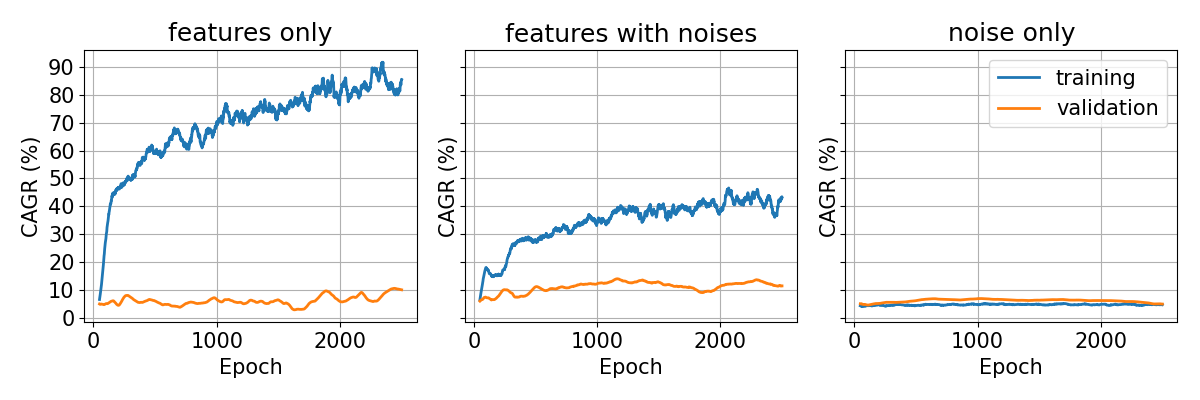
\includegraphics[width=15cm]{images/compare_noise.png}
  \caption{Comparison of using features with noise, features without noise, and noise only as states in terms of training/validation CAGR (moving average 50 Epochs)}
  \label{fig:noise_diagram}
\end{figure}

\subsection {Portfolio Builder}
The Portfolio Builder Build the portfolio from investments and actions
\subsection {Trading System}
The Trading System measures performances of the given portfolios
\subsection {Reward Provider}
The Reward Provider provides rewards based on the performances of the portfolio and investor preference.